\chapter{Ausarbeitung des Architekturkonzepts}
\label{chap:concept}
% Komponenten in dli anschauen und Übersetzungen für alle überlegen, dann beispielhaft von hand für verschiedene frameworks umsetzen und vergleichen -> chapter 3.
\section{Analyse bisheriger UI-Aufbau}
\subsection{DLI}
\subsection{VLC}

\section{React-Komponenten}
\subsection{Erste Layout-Überlegungen}
Zu Beginn erschien die zentrale Frage, wie  es technisch möglich ist, die Komponenten der Detailansicht vom Benutzer anpassbar anzuordnen. Eine naive Herangehensweise kann in Abbildung \ref{fig:layout_grid_test} gesehen werden. Umgesetzt wurde dies mit einem CSS-Grid (rote Umrandung) das entweder horizontal oder vertikal in zwei Hälften getrennt werden kann. Jede dieser Hälften stellt abermals ein CSS-Grid dar das beliebig zwischen Elterncontainern verschoben werden kann. Abstrakt handelt es sich bei diesem Ansatz um einen nicht balancierten binären Baum an dessen Endpunkten (Blätter) sich genau eine UI-Komponente (blaue Umrandung) befindet. Es wurde schnell klar dass diese Lösung in ihrer binären Form nicht flexibel genug ist um vorhandene Layouts abzubilden. Da ein Ausbau auf eine Struktur mit variabler Anzahl an Verzweigungen sehr komplex und zeitaufwändig gewesen wäre wurde der Ansatz gänzlich verworfen und nach einer Alternativen Lösung gesucht. \fixme{bessere erklärung und begründung warum nicht flexibel genug}

\begin{figure}
    \centering
    \captionsetup{justification=centering}
    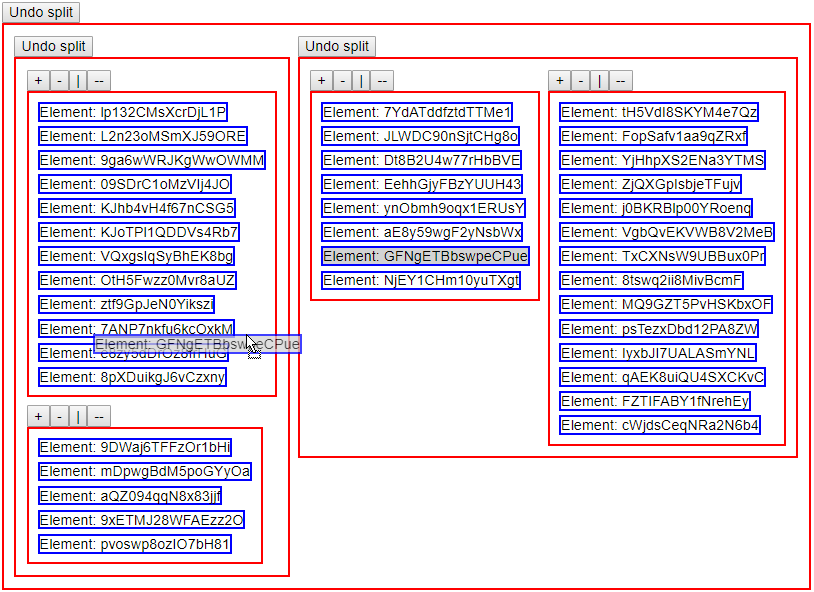
\includegraphics[width=\textwidth]{figures/layout_grid_test.png}
        \caption{Eigener Layout-Prototyp mit CSS-Grids}
        \label{fig:layout_grid_test}
\end{figure}

\subsection{Verwendung der Komponenten}
% => nicht nur Elemente sondern auch Anordnung wichtig!!
% Grid / Table
\subsection{Identifikation auf Server}
Um die UI-Elemente mit Daten aus der Datenbank zu befüllen muss eine entsprechende Identifikation möglich sein. Es wird vorausgesetzt dass diese eindeutige ID, ob sie aus Tabellennamen plus Spaltenname der Datenbank oder aus anderen Informationen besteht, zum Zeitpunkt der Übersetzung einer Ansicht bereits bekannt ist und mit ausgelesen werden kann. Bei Anfragen an den Server werden alle IDs der beteiligten Elemente mit an den Server übertragen, ebenso wie dieser bei Antworten immer die IDs der Elemente, für welche die Antwortdaten gedacht sind, sendet.

% moved from chapter 2:
% \subsubsection{copy of api contract from api itself}
% \subsubsection{no business logic in client}

% aktualitätsprüfung (evtl. konfigurierbar direkt über cmbt-server anstatt installation (keine versionskopplung vorausgesetzt))

% \subsubsection{FAQ / KB Artikel direkt suchbar (bereits als web-ressource verfügbar)}

\section{Tests und Continuous Integration}

% placeholder-komponenten für loading state und bei nicht mehr verfügbaren elementen
